\documentclass[aip, jcp, reprint, onecolumn, nofootinbib]{revtex4-2}

\bibliographystyle{apsrev4-2}

\usepackage{physics}
\usepackage{amsmath}
\usepackage{amssymb}
\usepackage{mathtools}
\usepackage{graphicx}
\usepackage{dcolumn}
\usepackage[colorlinks=true, linkcolor=black, urlcolor=blue, citecolor=black, anchorcolor=black]{hyperref}

%supplementary figs
\renewcommand{\thefigure}{S\arabic{figure}}
\renewcommand{\thetable}{S\arabic{table}}
\renewcommand\theequation{S\arabic{equation}}
\renewcommand*{\thepage}{S\arabic{page}}

\graphicspath{{"figures/"}}
\begin{document}
%Title of paper
\title{Supporting Information for Coherent IR-Hyper-Raman Four Wave Mixing Spectroscopy}


\author{Ryan P. McDonnell} 
\author{Daniel D. Kohler}
\author{John C. Wright} \email{wright@chem.wisc.edu}

\affiliation{Department of Chemistry, 
        University of Wisconsin - Madison, 
        Madison, Wisconsin 53706, 
        United States of America}

\date{\today}

\maketitle
\tableofcontents
\clearpage


\section{Evaluating Herzberg-Teller Integrals for Harmonic Wells of Identical Curvature}
In this section, we discuss the evaluation of Herzberg-Teller integrals when the ground and first excited state are harmonic wells of identical curvature.\cite{HerzbergTeller1933}
% We note that Myers et al. have developed a general expression to evaluate Franck-Condon factors for two displaced harmonic wells of differing curvature,\cite{Myers1982} 
We investigate the one dimensional case using the Hamiltonian described in the main text, $H = H_g |g) \left(g| + H_e |e\right) (e|$, where
\begin{subequations}\label{Hamiltonian}
	\begin{equation}
		H_g = \frac{\hbar \omega }{2} \left(p^2 + q^2 \right)
	\end{equation}
	and
	\begin{equation}
		H_e = \frac{\hbar \omega }{2} \left(p^2 +  (q-\Delta)^2 \right) + \hbar \omega_{eg}.
	\end{equation} 
\end{subequations}
Here, $p,q$ are the dimensionless conjugate normal mode coordinates, $\hbar\omega_{eg}$ is the energy difference between $H_e$ and $H_g$, and $\Delta$ is the dimensionless offset of the excited state surface relative to the ground state.
The Hamiltonians are the well-known quantum harmonic oscillator, and their solutions are
\begin{equation}
	\psi_m(q) = \langle q | m \rangle = N_m H_m(q) \exp(-q^2/2),
\end{equation}
where $N_m = (m! \ 2^m \pi^{\frac{1}{2}})^{-\frac{1}{2}}$ is the normalization factor and $H_m$ is the $m^{th}$ Hermite Polynomial.\cite{RN230}

For an $n$-quantum excited state vibration $| \tilde{n} \rangle$, and a $m$-quantum ground state vibration $| \tilde{m} \rangle$, the $k^{th}$-order vibrational coupling term is
\begin{equation}
	\begin{split}
			\mel{\tilde{n}}{q^k}{m} &= \int_{-\infty}^\infty \mathrm{d}q \ \psi^*_n(q-\Delta) q^k \psi_m(q)\\
			&= \int_{-\infty}^\infty \mathrm{d}q \ N_n H_n(q-\Delta) \exp(-\frac{(q - \Delta)^2}{2}) q^k N_m H_m(q) \exp(-\frac{q^2}{2}). \\
			&= N_n N_m \exp(-\frac{\Delta^2}{2}) \int_{-\infty}^\infty \mathrm{d}q \ H_n(q-\Delta) q^k H_m(q) \exp(-q^2 + q\Delta)
		\end{split}\label{key}
\end{equation}
The integral corresponds to Franck-Condon matrix elements for $k=0$ and Herzberg-Teller matrix elements for $k=1$.

The matrix elements of \autoref{key} can be computed numerically, but analytic forms of the integral also exist. 
Due to the polynomial nature of $H_v(q)$, evaluation of \autoref{key} reduces into evaluating sums of integrals of the form
\begin{equation}\label{integral}
	\int_{-\infty}^\infty \mathrm{d}q \ q^w \exp(-q^2 + q\Delta)
\end{equation}
When $w=0$, the result follows by completing the square:\footnote{$\int_{-\infty}^{\infty} \mathrm{d}x \exp(-(x-a)^2) = \sqrt{\pi}$}
\begin{equation}
	\begin{split}
		\int_{-\infty}^\infty \mathrm{d}q \exp(-q^2 + q\Delta) &= \int_{-\infty}^\infty \mathrm{d}q \exp(-(q^2 - q\Delta +\frac{\Delta^2}{4} - \frac{\Delta^2}{4}))\\
		&= \exp(-\frac{\Delta^2}{4}) \int_{-\infty}^\infty \mathrm{d}q \exp(-(q - \frac{\Delta}{2})^2) \\
		&= \sqrt{\pi} \exp(-\frac{\Delta^2}{4})
	\end{split}
\end{equation}
 For $w \neq 0$, \autoref{integral} is evaluated through repeated use of a well-known Gaussian identity
\begin{equation}\label{identity}
	\int_{-\infty}^\infty \mathrm{d}q \ q^w \exp(-q^2 + q\Delta) = \partial_{\Delta} \int_{-\infty}^\infty \mathrm{d}q \ q^{w-1} \exp(-q^2 + q\Delta)
\end{equation}

We now have the background needed to calculate $\mel{\tilde{1}}{q}{0}$ for an arbitrary offset $\Delta$.
Using $H_0(q) = 1$ and $H_1(q) = 2q$,
\begin{equation}\label{HT10}
	\begin{split}
		\mel{\tilde{1}}{q}{0} &= N_1 N_0 \exp(-\frac{\Delta^2}{2}) \int_{-\infty}^\infty \mathrm{d}q \ 2(q - \Delta) q \exp(-q^2 + q\Delta)\\
		&= 2N_1 N_0 \exp(-\frac{\Delta^2}{2}) \left( \int_{-\infty}^\infty \mathrm{d}q \ q^2 \exp(-q^2 + q\Delta) + \Delta \int_{-\infty}^\infty \mathrm{d}q \ q \exp(-q^2 + q\Delta) \right)
	\end{split}
\end{equation}
Both integrals can be evaluated using \autoref{identity}:
\begin{subequations}\label{evalGaussians}
	\begin{equation}
		\begin{split}
					\int_{-\infty}^\infty \mathrm{d}q \ q \exp(-q^2 + q\Delta) &= \partial_{\Delta} \left(\sqrt{\pi} \exp(\frac{\Delta^2}{4})\right)\\
					& = \sqrt{\pi} \frac{\Delta}{2} \exp(\frac{\Delta^2}{4})
		\end{split}
	\end{equation}
	\begin{equation}
	\begin{split}
		\int_{-\infty}^\infty \mathrm{d}q \ q^2 \exp(-q^2 + q\Delta) &= \partial_{\Delta} \left(\sqrt{\pi} \left(\frac{\Delta}{2} \exp(\frac{\Delta^2}{4})\right)\right)\\
		& =\sqrt{\pi} \left(\frac{1}{2}\exp(\frac{\Delta^2}{4}) + \frac{\Delta^2}{4} \exp(\frac{\Delta^2}{4})\right)
	\end{split}
\end{equation}
\end{subequations}
Substituting the results of \autoref{evalGaussians} into \autoref{HT10}, 
\begin{equation}
	\mel{\tilde{1}}{q}{0} = \sqrt{\frac{1}{2}} (1 - \frac{\Delta^2}{2}) \exp(\frac{-\Delta^2}{4})
\end{equation}
The evaluation of other Herzberg-Teller integrals is analogous. 


\pagebreak
\section{Impact of displacement, resonance frequencies, and vibronic linewidth and on HDFG Spectra}
\begin{figure}[!htbp]
	\centering
	\includegraphics[width=6.675in]{figures/fcht.png}
	\caption{Plots of select (a) Franck-Condon factors and (b) Herzberg-Teller integrals relevant to this manuscript as a function of offset, $\Delta$.} 
	\label{fig:fcht}
\end{figure}

\begin{figure}[!htbp]
	\centering
	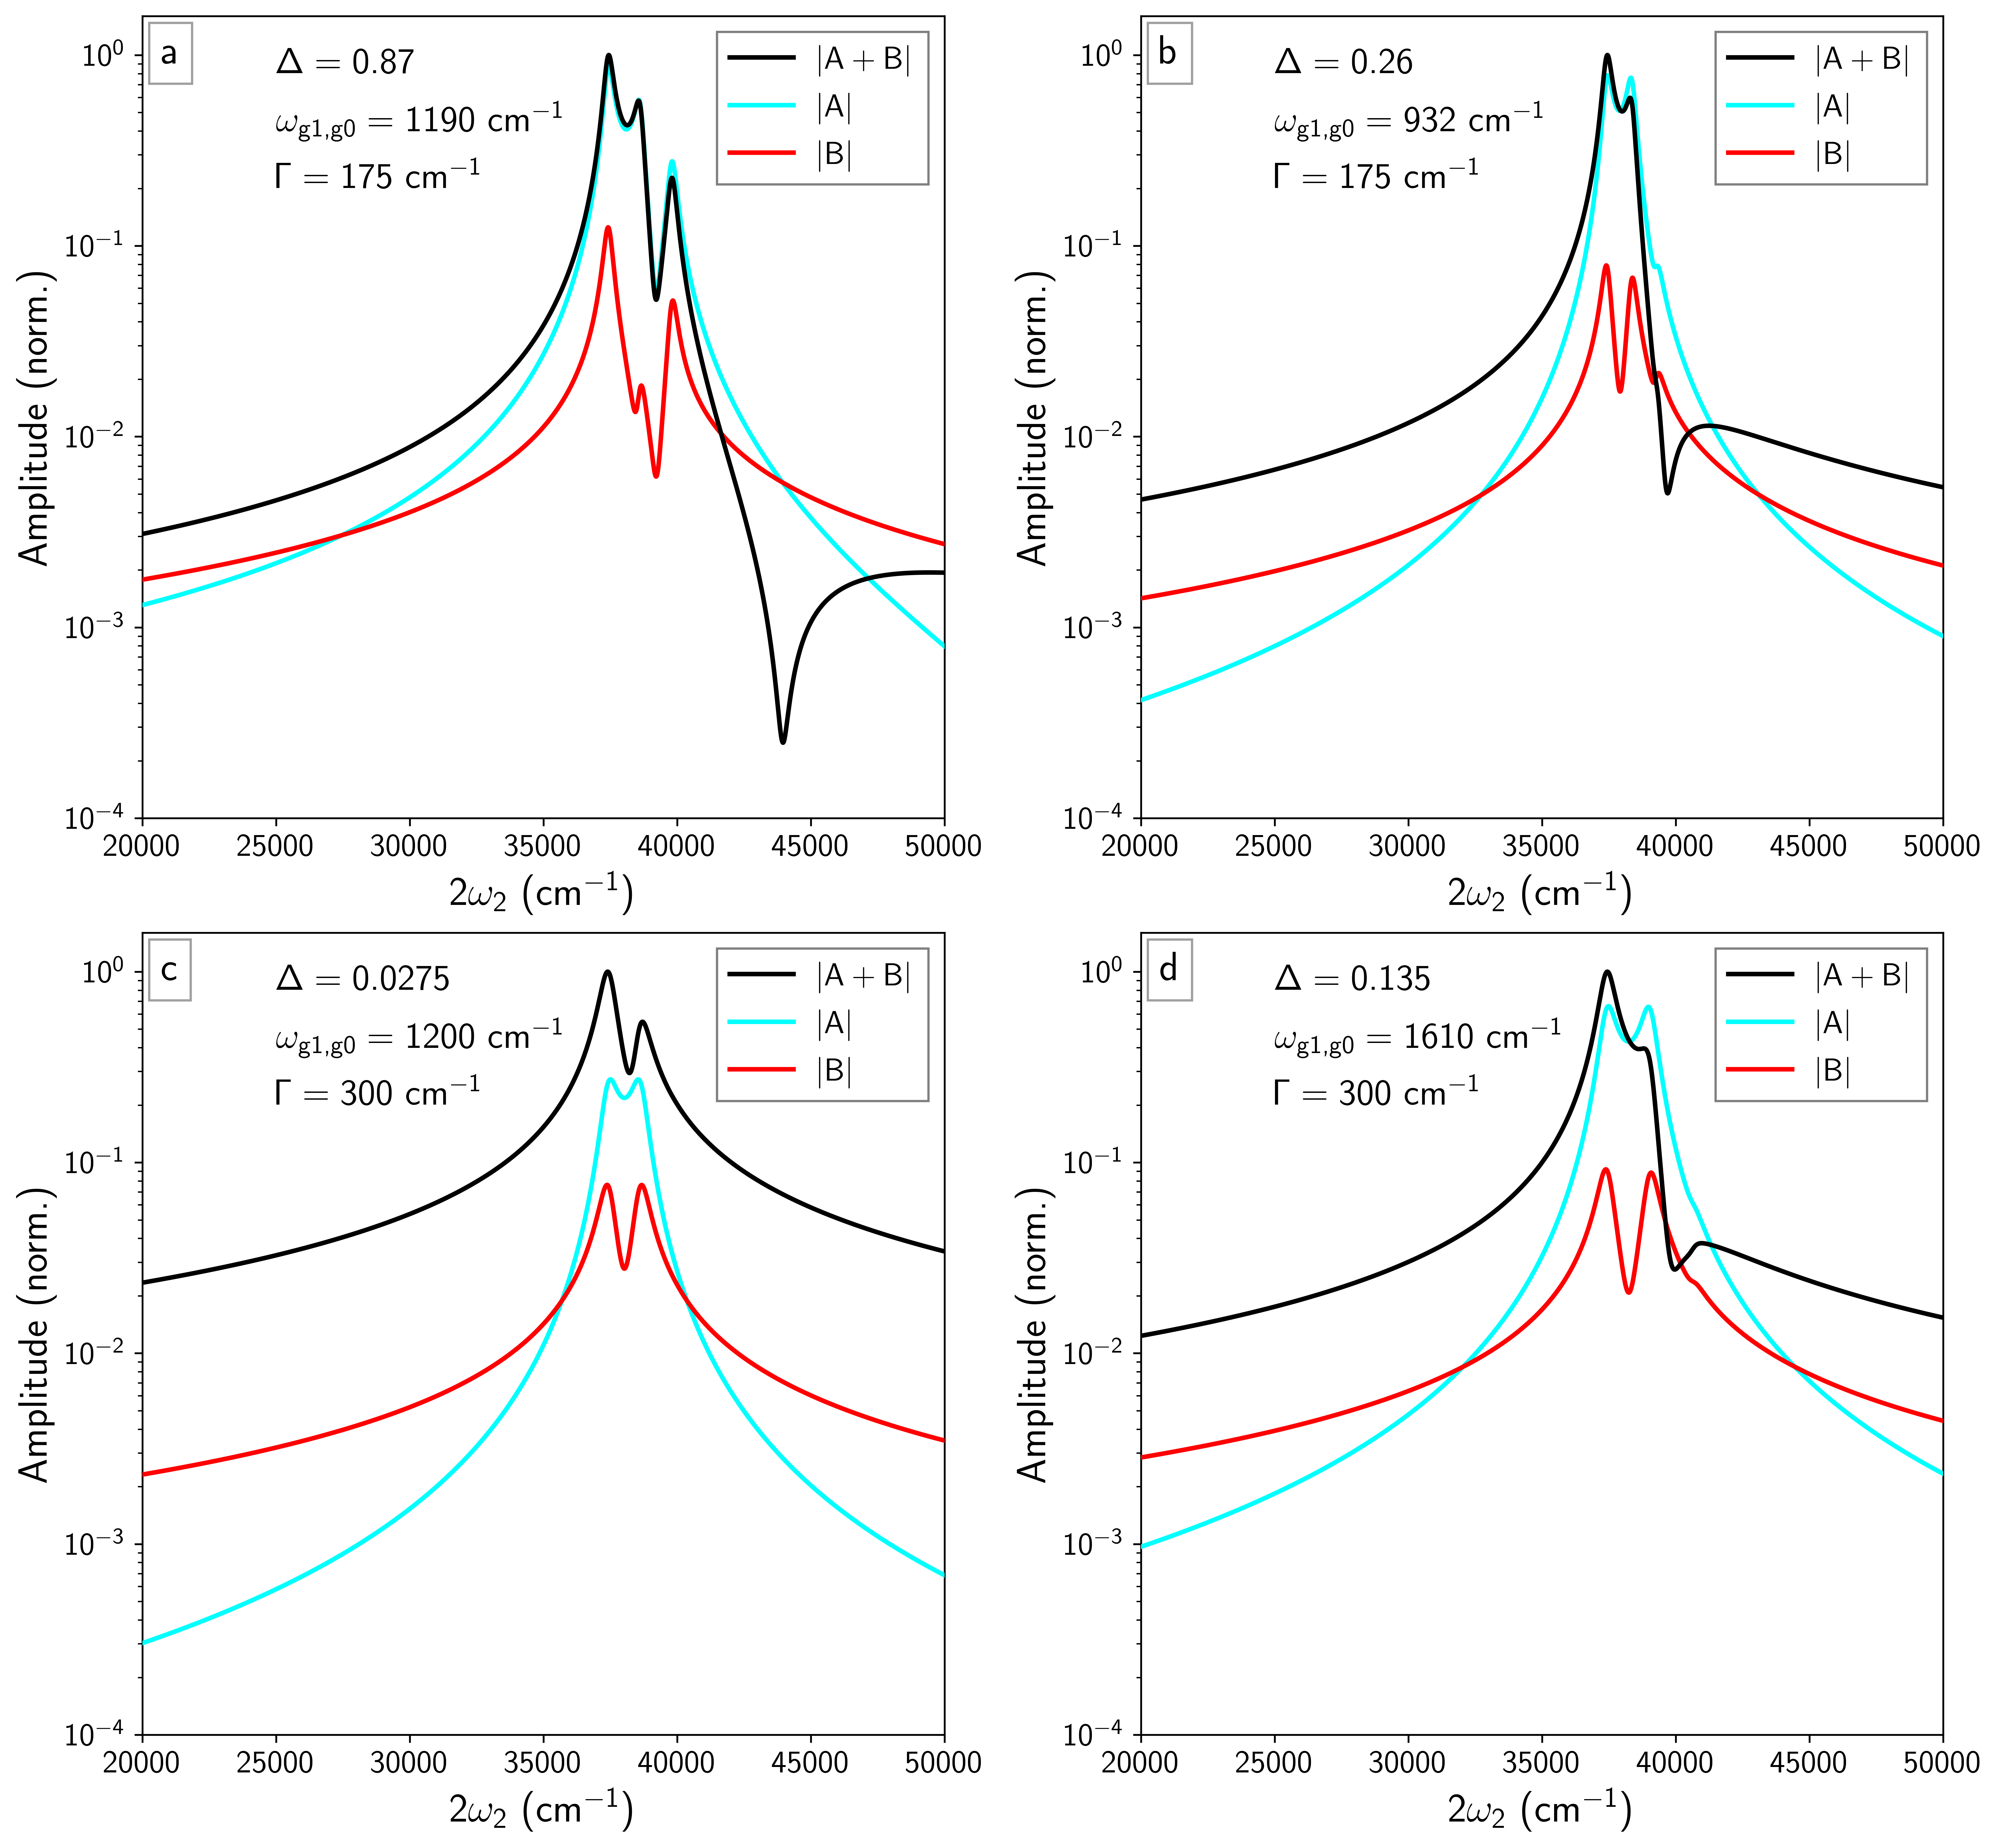
\includegraphics[width=6.675in]{figures/changedelta.png}
	\caption{The impact of offset, vibrational resonance, and linewidth on HDFG spectra. Parameters for (a,b) follow from Myers et al., whereas parameters for (c,d) follow from Brennan et al.\cite{Myers1982, Brennan2024}} 
	\label{fig:chgdelta}
\end{figure}

\pagebreak

In the main text, the potential well offset ($\Delta$) was taken as $\Delta = 0.5$.
Here, we vary $\Delta$ to investigate its impact on the structure of the $\abs{A+B}$ spectrum.
The dependence of relevant Franck-Condon factors and Herzberg-Teller factors on displacement are plotted in \autoref{fig:fcht} as a function of offset, $\Delta$.
\autoref{fig:fcht} shows how different displacements, vibrational frequencies, and vibronic linewidths will alter the vibronic spectrum.

It is clear from \autoref{fig:fcht} that the HDFG spectrum will have a significant dependence upon $\Delta$, even for small deviations from complete overlap. 
To this end, we plot the impact of resonance frequency and offset on the HDFG spectrum \autoref{fig:chgdelta}, using values reported by Myers et al. and Brennan et al. \cite{Myers1982, Brennan2024}
In this section, we take $\omega_{eg}$ = $37340$ cm$^{-1}$ and vary the offset ($\Delta$), vibrational frequency ($\omega_{g1,g0}$), and linewidth ($\Gamma$) as noted in the figure.

\pagebreak

\section{Evaluating impact of inhomogeneity on HDFG output}
In this section, the integral
\begin{equation}\label{generalcontour}
	\begin{split}
		\gamma_{ijkl} &= \int_{-\infty}^\infty \mathrm{d}\xi P(\xi) \gamma_{ijkl}(\xi)\\
		&= \frac{\sigma}{\pi}\int_{-\infty}^\infty \mathrm{d}\xi \frac{1}{\sigma^2 + \xi^2} \frac{\eta_{ijkl}}{\left(\Delta_{ga} - \xi\right)\left(\Delta_{ba}+ c\xi\right)} \\
		&= \frac{\eta_{ijkl} \sigma}{\pi} \int_{-\infty}^\infty \mathrm{d}\xi\frac{1}{(\xi + i\sigma)(\xi - i\sigma)} \frac{1}{\Delta_{ga} - \xi} \frac{1}{\Delta_{ba} + c\xi}\\
	\end{split}
\end{equation}
is evaluated for $c=-1$ (electronic state and vibrational state energy fluctuations are anti-correlated) $c=1$ (electronic state and vibrational state energy fluctuations are correlated).

\subsection{Anti-correlated Modes}
For anti-correlated modes ($c = -1$), the poles ($\xi_k$) are situated in the complex plane as shown in \autoref{fig:contours}a.
Since \autoref{generalcontour} is evaluated along the real axis, one can choose to evaluate the contour in the upper or lower half of the complex plane.
In other words, we can choose the contour which wraps around the least number of poles.
For c = -1, there are four poles: $\pm i \sigma, \Delta_{ga}, \Delta_{ba}$. 
The contour that wraps the upper half of the complex plane has only one pole, $i \sigma$; as such, we choose to evaluate \autoref{generalcontour} in the upper half of the complex plane for the case of anti-correlated modes, as it contains the least number of poles.
Using the residue theorem, we see
\begin{widetext}
	\begin{equation}
		\begin{split}
			\int_{-\infty}^\infty \mathrm{d}\xi P(\xi) \gamma_{ijkl}(\xi) &= 2\pi i \sum_k \lim_{\xi \rightarrow \xi_k} P(\xi) \gamma_{ijkl}(\xi) (\xi - \xi_k)\\
			&= 2\pi i \frac{\eta_{ijkl} \sigma}{\pi} \lim_{\xi \rightarrow i\sigma} \frac{1}{(\xi + i\sigma)(\xi - i\sigma)} \frac{1}{\Delta_{ga} - \xi} \frac{1}{\Delta_{ba} - \xi} (\xi - i \sigma)\\
			&= 2 \eta_{ijkl} \sigma i \lim_{\xi \rightarrow i\sigma} \frac{1}{\xi + i\sigma} \frac{1}{\Delta_{ga} - \xi} \frac{1}{\Delta_{ba} - \xi}\\
			&= 2\eta_{ijkl} \sigma i \frac{1}{2i\sigma} \frac{1}{\Delta_{ga} - i\sigma} \frac{1}{\Delta_{ba} - i\sigma}\\
			&= \frac{\eta_{ijkl}}{\left(\Delta_{ga}-i\sigma\right)\left(\Delta_{ba}-i \sigma\right)}\\
		\end{split}
	\end{equation}
\end{widetext}


\subsection{Correlated Modes}
For correlated modes, the poles are situated in the complex plane as shown in \autoref{fig:contours}b.
It is clear that no matter which contour is chosen, the contour will envelop two poles.
We choose to evaluate along the contour in the bottom half of the complex plane (see \autoref{fig:contours}b), where the poles are $\{-i\sigma, \Delta_{ga}\}$.
Since the $\xi_k$ are nondegenerate, we see
\begin{widetext}
	\begin{equation}
		\begin{split}
			\int_{-\infty}^\infty \mathrm{d}\xi P(\xi) \gamma_{ijkl}(\xi) &= 2\pi i \sum_k \lim_{\xi \rightarrow \xi_k} P(\xi) \gamma_{ijkl}(\xi) (\xi - \xi_k)\\
			&= 2\pi i \frac{\eta_{ijkl} \sigma}{\pi}  \lim_{\xi \rightarrow -i\sigma} \frac{1}{(\xi + i\sigma)(\xi - i\sigma)} \frac{1}{\Delta_{ga} + \xi} \frac{1}{\Delta_{ba} - \xi} \left(\xi + i \sigma\right) \\ 
			&+ 2\pi i \frac{\eta_{ijkl} \sigma}{\pi} \lim_{\xi \rightarrow \Delta_{ga}} \frac{1}{(\xi + i\sigma)(\xi - i\sigma)} \frac{1}{\Delta_{ga} - \xi} \frac{1}{\Delta_{ba} - \xi} \left(\xi - \Delta_{ga}\right)\\
			&= 2 \eta_{ijkl} i \sigma \left(\frac{1}{2 i \sigma} \frac{1}{-i \sigma - \Delta_{ga}} \frac{1}{\Delta_{ba} - i\sigma} \right) - 2\eta_{ijkl} i \sigma \left(\frac{1}{\sigma^2 + \Delta_{ga} ^2} \frac{1}{\Delta_{ga} + \Delta_{ba}} \right)\\
			&= -\frac{\eta_{ijkl}}{\Delta_{ga} + i \sigma} \left(\frac{1}{\Delta_{ba} - i \sigma} + \frac{2i\sigma}{(\Delta_{ga} - i \sigma)(\Delta_{ga} + \Delta_{ba})}\right)\\
		\end{split}
	\end{equation}
\end{widetext}


\begin{figure}[!htbp]
	\centering
	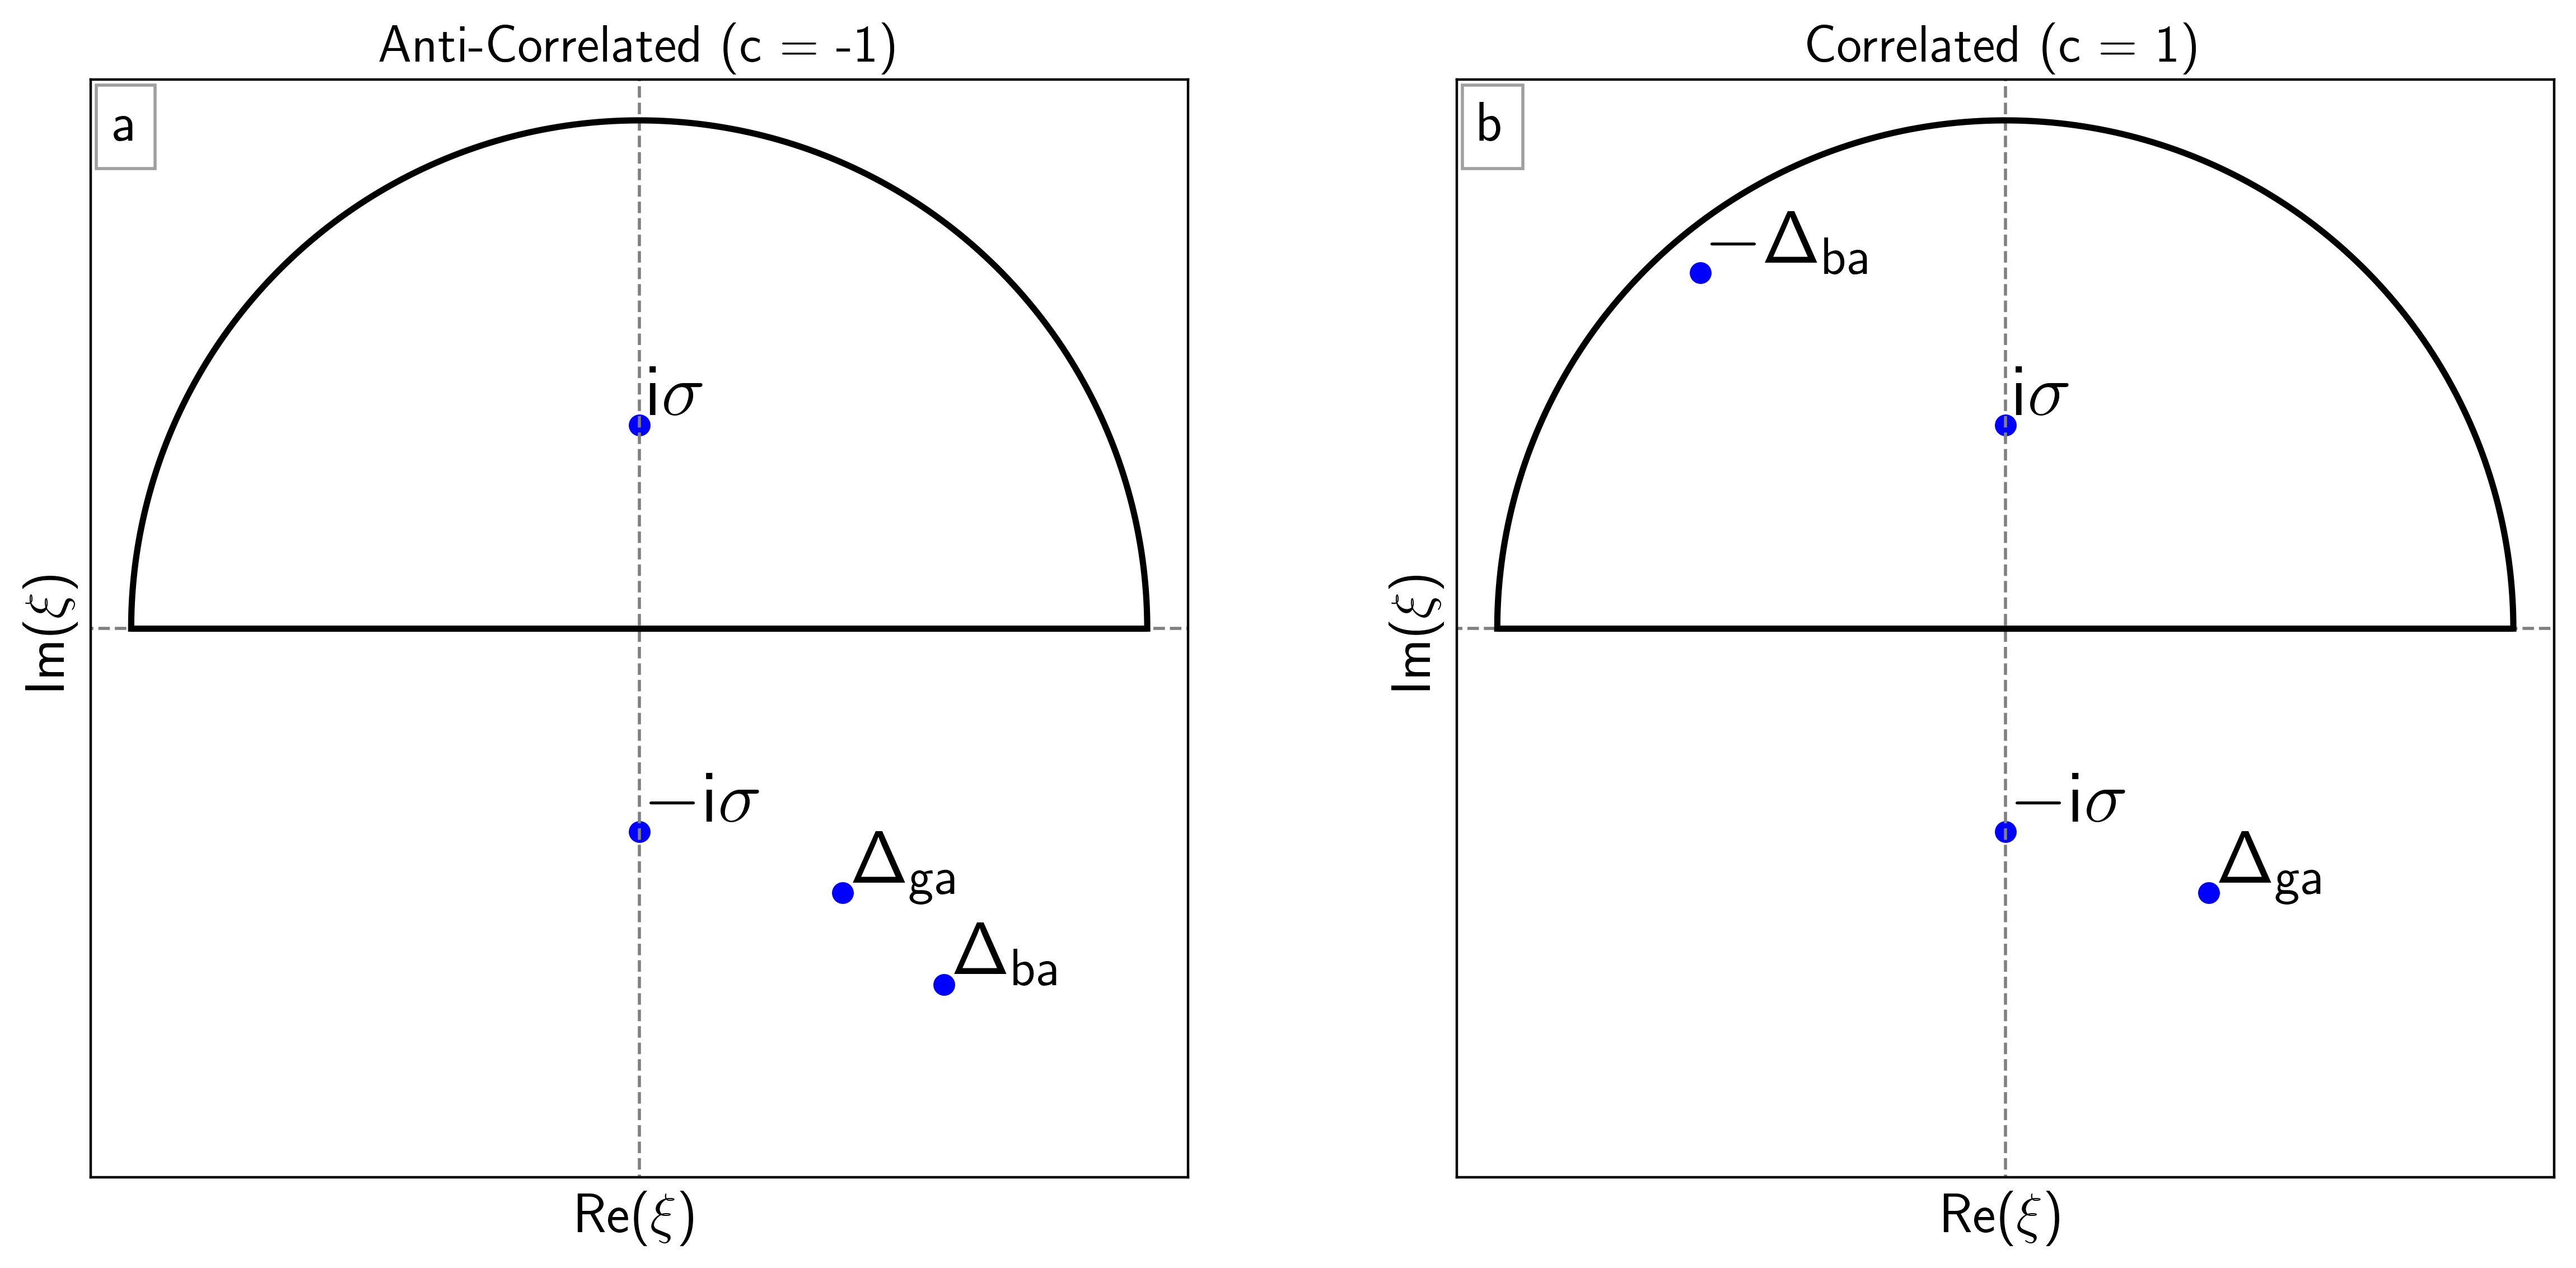
\includegraphics[width=6.675in]{figures/corr_contour.png}
	\caption{Poles (blue dots) and contours (black line) used to evaluate \autoref{generalcontour} for (a) anti-correlated and (b) correlated modes.} 
	\label{fig:contours}
\end{figure}


\section{References}
% Create the reference section using BibTeX:
\bibliography{library.bib}

\end{document}
%


